%%%%%%%%%%%%%%%%%%%%%%%%%%%%%%%%%%%%%%%%%
% Simple Sectioned Essay Template
% LaTeX Template
%
% This template has been downloaded from:
% http://www.latextemplates.com
%
% Note:
% The \lipsum[#] commands throughout this template generate dummy text
% to fill the template out. These commands should all be removed when 
% writing essay content.
%
%%%%%%%%%%%%%%%%%%%%%%%%%%%%%%%%%%%%%%%%%

%----------------------------------------------------------------------------------------
% PACKAGES AND OTHER DOCUMENT CONFIGURATIONS
%----------------------------------------------------------------------------------------

\documentclass[12pt]{article} % Default font size is 12pt, it can be changed here
\usepackage[utf8]{inputenc} % utf8 support
\usepackage[T1]{fontenc}
\usepackage[official]{eurosym}
\usepackage[font=small,skip=0pt]{caption}
\usepackage{geometry} % Required to change the page size to A4
\usepackage{gensymb}
\geometry{a4paper} % Set the page size to be A4 as opposed to the default US Letter

\usepackage{graphicx} % Required for including pictures

\usepackage{float} % Allows putting an [H] in \begin{figure} to specify the exact location of the figure
\usepackage{wrapfig} % Allows in-line images such as the example fish picture

\usepackage{subfig}
\usepackage[style=numeric, backend=biber, sorting=none]{biblatex}
\bibliography{kilgarvan.bib}

\linespread{1.2} % Line spacing

%\setlength\parindent{0pt} % Uncomment to remove all indentation from paragraphs

\graphicspath{{./img/}} % Specifies the directory where pictures are stored


\begin{document}

%----------------------------------------------------------------------------------------
% TITLE PAGE
%----------------------------------------------------------------------------------------

\begin{titlepage}
  \newcommand{\HRule}{\rule{\linewidth}{0.5mm}} % Defines a new command for the horizontal lines, change thickness here

  \center % Center everything on the page

  \textsc{\LARGE University College Cork}\\[1.5cm] % Name of your university/college
  \textsc{\Large Wind Energy}\\[0.5cm] % Major heading such as course name
  % \textsc{\large Minor Heading}\\[0.5cm] % Minor heading such as course title

  \HRule \\[0.4cm]
  { \huge Kilgarvan Wind Farm Visit 28-10-2015}\\[0.5cm] % Title of your document
  \HRule \\[1.5cm]

  \begin{minipage}{0.4\textwidth}
  \begin{flushleft} \large
  \emph{Author:} Peter \textsc{Armstrong} \\% Your name 
  \emph{Student ID:} 115224113
  \end{flushleft}
  \end{minipage}
  ~
  \begin{minipage}{0.4\textwidth}
  \begin{flushright} \large
  % \emph{Supervisor:} \\
  % Dr. James \textsc{Smith} % Supervisor's Name
  \end{flushright}
  \end{minipage}\\[4cm]

  {\large \today}\\[3cm] % Date, change the \today to a set date if you want to be precise

  \vfill % Fill the rest of the page with whitespace

% itemize changes
\newlength{\wideitemsep}
\setlength{\wideitemsep}{.5\itemsep}
\addtolength{\wideitemsep}{-7pt}
\let\olditem\item
\renewcommand{\item}{\setlength{\itemsep}{\wideitemsep}\olditem}

\end{titlepage}

%----------------------------------------------------------------------------------------
% TABLE OF CONTENTS
%----------------------------------------------------------------------------------------

% \tableofcontents % Include a table of contents

% \newpage % Begins the essay on a new page instead of on the same page as the table of contents 

%----------------------------------------------------------------------------------------
% INTRODUCTION
%----------------------------------------------------------------------------------------

\section{Site Description} % Major section

The Kilgarvan wind farms are situated on the western side of the Derrynasaggart mountains, Co. Kerry. In the area, there is a cluster of wind farms. This group of wind farms have been built over the last 10 years.

Three of the farms on this site are operated by Brookfield Renewables. Brookfield are an international company that bought Bórd Gáis' wind farm assets in 2014 \cite{silicon_republic}. Brookfield operate around 15\% of the installed wind capacity in Ireland.
The farm that we visited is known as Kilgarvan/Coomagearlahy I and Coomagearlahy III \cite{iwea}.

\begin{figure}[h]
  \begin{center}
    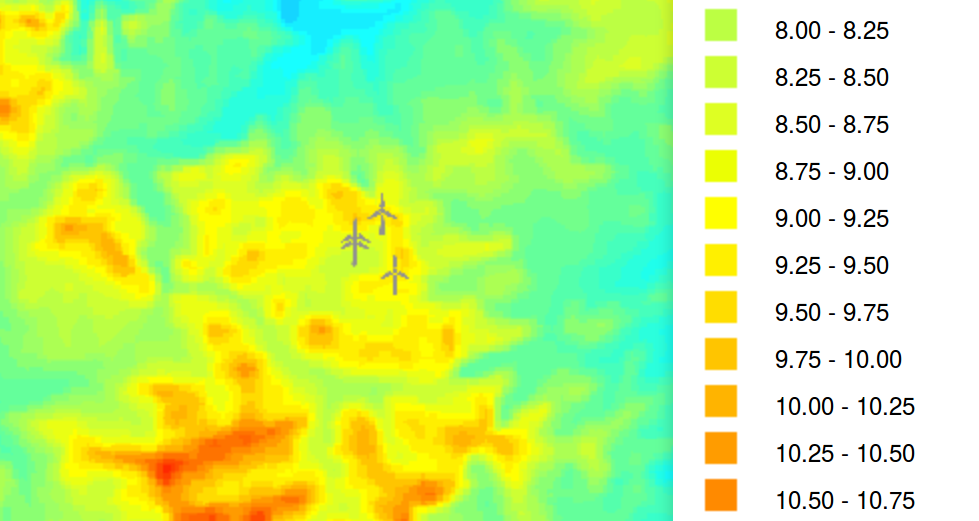
\includegraphics[width=1\textwidth]{seai_wind_atlas_kilgarvan}
  \end{center}
  \caption{Wind speed at 75m - SEAI Wind Atlas - Kilgarvan Area}
\end{figure}

According to the SEAI Wind Atlas \cite{seai_atlas}, the area has some of the best onshore wind conditions in Ireland. Average wind speeds at 75m height are between 8 - 10 m/s. The wind conditions are also relatively consistent, with a Weibull k modulus of 2 - 2.5.

The terrain can be described as complex, mountainous terrain - there are large depressions and hills in the area. This will affect the vertical wind profile, power output of turbines and choice of turbine design.
Depending on wind direction, the terrain effects will differ. 
The turbines are sited on the south western hillside. If the wind blows from the prevailing south west direction, the turbines will experience a speed up effect due to acceleration over the hill.
If the wind is blowing from a northerly or easterly direction, the turbines will be in the lee of the hills and will experience lower wind speeds and more turbulent conditions.


\subsection{Access Route}
Access to Kilgarvan windfarm is off the N22. 
The first electricity infrastructure visible is an Eirgrid/ESB operated substation just off the main road. This substation connects directly to the national 110kV grid.
An access road winds from the N22 to the wind farm site. The road passes through both rocky and bog areas. Some cutting away of bog and rock was necessary to build the road. Turbines were transported to the site in sections up to 45m length on this road so it has a gentle incline and wide turns.

The area on the lee side of the hills is forested. Although the land is owned by the wind farm operator, Brookfield, the forestry is managed by Caoilte.
There is no forestry on the windward side of the hills where the wind turbines are located.
Road resurfacing works were recently completed to improve the access route.

% research building roads through bogs


\section{Technology}
\subsection{Wind Machines}

There are two types of wind turbine installed on the site. Both types are large, variable speed, horizontal axis wind turbines.

The Kilgarvan / Coomagearlaghy site has 15 Vestas V90 turbines. The site has a capacity of 42.5MW and was commissioned in 2007 \cite{iwea}.
The Vestas V90 is a 3MW turbine. The blades are made from lightweight carbon fibre and glass fibre composite materials. The nacelle and tower are also designed to reduce weight. The light weight reduces transportation, installation and foundation costs \cite{v90-3.0}. The V90 has a rotor diameter of 90m.
Vestas \cite{v90-3.0} describe the V90 as 'a great choice for high and medium wind sites with high turbulence'. 
According to Vestas, the cut in wind speed of the V90 is 3.5m/s and the cut out wind speed is 25m/s. The rated wind speed is 15m/s.
The V90 can be used with a variety of different tower heights, but at Kilgarvan it is mounted on a 75m tower. The V90 was originally designed for offshore use. The turbines at Kilgarvan were the first V90 turbines installed onshore.

\begin{figure}[h]
  \begin{center}
    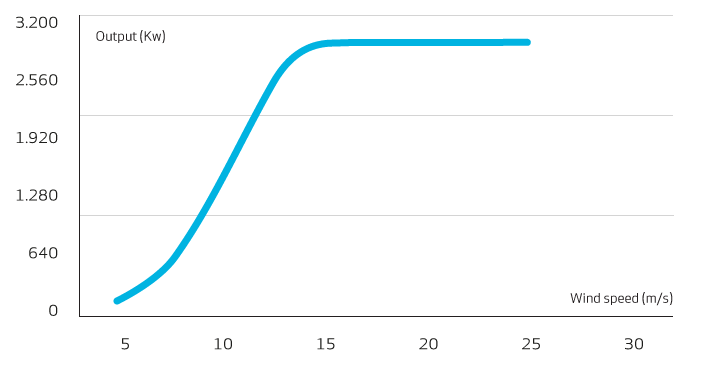
\includegraphics[width=1\textwidth]{PowerCurveV9030MW}
    \hbox{\scriptsize Image credit: Vestas \cite{v90-3.0}}
  \end{center}
  \caption{Vestas V90 Power Curve}
  \label{fig:v90powercurve}
\end{figure}

Figure \ref{fig:v90powercurve} shows the power curve of the Vestas V90. This shows the cut in, cut out and rated wind speeds for the turbine.


The neighbouring Coomagearlahy III site was commissioned in 2009 and has a capacity of 30MW. It has 13 Nordex N90 turbines. The Nordex N90 is a 2.5MW turbine with a 90m rotor diameter. It has similar design specifications as the Vestas V90. Nordex \cite{n90} describe the N90 as 'As an all-round turbine ... (that) can be deployed at strong-wind sites'.
According to Nordex, the cut in wind speed for the N90 is 3m/s. The cut out speed is 25m/s.


Both turbines meet the IEC-1A certification. Turbines with this certification are designed for average wind speeds of around 10m/s with extreme 50 year gusts of 50m/s \cite{burton_wind_2001}. The A certification means these turbines are suitable for use in areas of high turbulence.

Both turbines have variable pitch controls to change the pitch of the blades. This is used to regulate the power capture and speed of the rotor. In high wind conditions, the turbines are depowered by feathering the blades. In extreme conditions the blades can be feathered to 90\degree to stop the turbine. If even one blade is feathered like this, the turbine will loose power and a holding disc brake can be applied to the shaft.

Alternatively, if the wind speed is below the rated wind speed, the turbine can be powered up by increasing the angle of attack of the blades.
The Noredex turbine uses an electrical pitch control system. Each turbine has battery backup for the pitch control system.
The Vestas machines use a hydraulic pitch system that does not require battery backup.
The pitch of the blades is managed automatically by the turbine control system.

The blades on the Vestas machines appear to be swept back significantly. The Nordex blades appear straighter. There was a noticeable twist along the length of the blades. This twist is designed in to accommodate the change in apparent wind speed along the length of the blades. Figure \ref{fig:vestasrotor} shows Vestas rotor. Note the swept back blades and twist of the blades.

\begin{figure} % Inline image example
  \begin{center}
    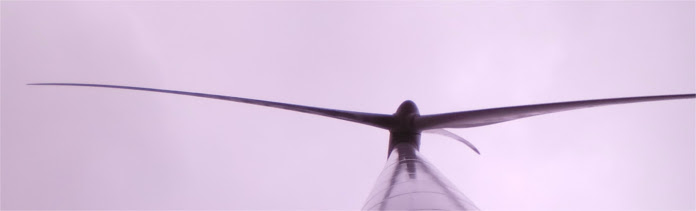
\includegraphics[width=1\textwidth]{turbine_blades}
  \end{center}
  \caption{Vestas V90 Rotor}
  \label{fig:vestasrotor}
\end{figure}

Some machines are on better sites than others. Some machines are located in depressions, or shadowed by the hillside if the wind is blowing in a particular direction. The power output of the turbines can vary significantly depending on their location. The best performing machine is a Vestas machine on the top of the hill. The worst performing machines are Nordex machines at the bottom of the hill.
The worst performing machines can generate as little as 40\% of the power as the best performers. This is expected and is taken into account at the design stage.


A further 5 N90 turbines are planned for the site. Turbines cost approximately \euro2.5 million and have a 25 year operational lifetime. The cost of the turbines is expected to be paid back in 8 years.
\begin{figure}[h]
	\begin{center}
	  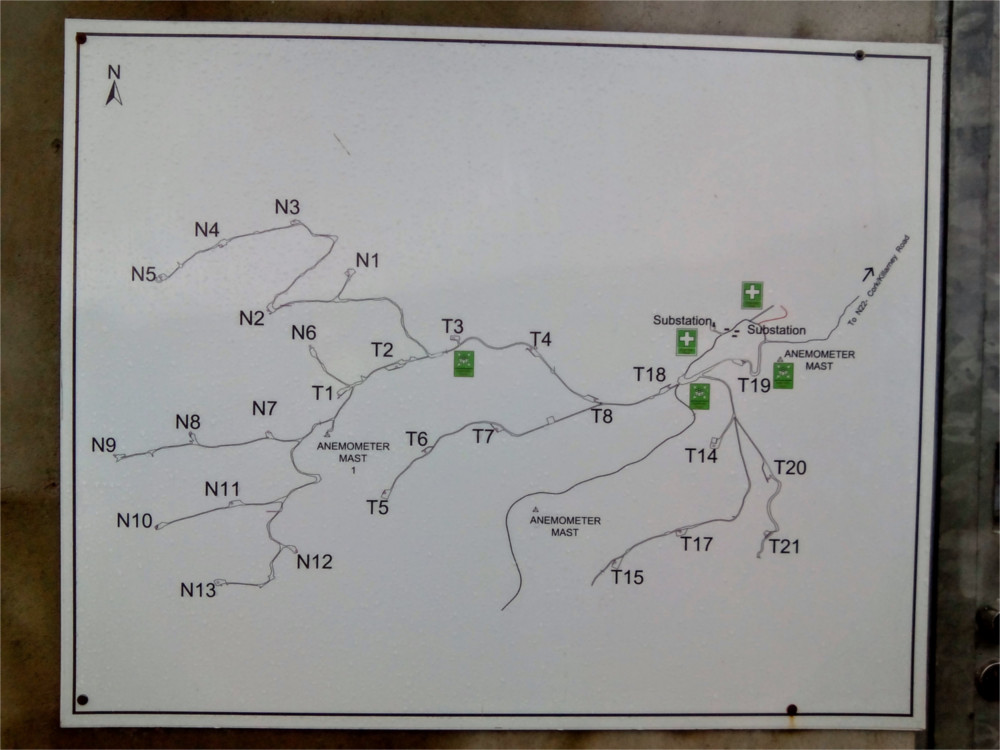
\includegraphics[width=1\textwidth]{kilgarvan_layout}
	\end{center}
	\caption{Farm Layout - N indicates Nordex, T indicates Vestas}
  \label{fig:sitemap}
\end{figure}

Each turbine has an access door at the base of the tower. Inside, there is a turbine control system, voltage converter, ring main unit (RMU) and a ladder and lift to access the nacelle. The RMU acts as a fuse or circuit breaker in case of issues with the grid or turbine. Ascending the turbine tower in the lift takes 2 minutes.

\subsection{Wind Measurement}
There are three anemometer masts on the site. They are spread out to different areas and are at different elevations. The positions of the anemometers can be seen in figure \ref{fig:sitemap}.

\subsection{Electrical Infrastructure}
The turbines generate electricity at 1000V, 50Hz. The voltage is stepped up to 20kV at the bottom of the turbine where it is connected to the local on-site grid. The voltage is stepped up to 110kV at the Brookfield operated substation at the top of the site.

\begin{figure}[H]
  \begin{center}
    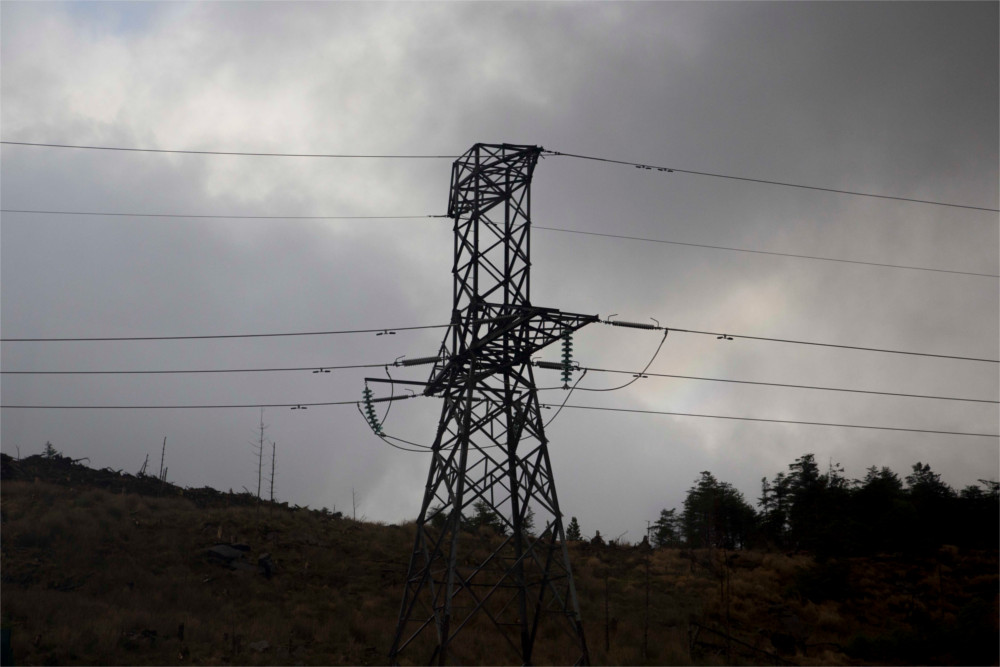
\includegraphics[width=1\textwidth]{pylons}
  \hbox{\scriptsize Photo credit: Aldert Otter}
  \end{center}
  \caption{Pylon carrying 110kV electricity lines}
  \label{fig:pylons}
\end{figure}
The on-site grid between the turbines and the substation is not visible and can be assumed to use underground cables.
The Brookfield substation is connected to the ESB substation with a series of wooden and metal pylons. The pylons, as shown in figure \ref{fig:pylons}, carry five cables - one for each phase of the 3-phase electricity being generated, one ground cable and one communications fibre optic cable.


\section{Operations and Conditions}

\subsection{Maintenance Requirements}
Wind machines need periodic maintenance to keep them operating safely and efficiently. 
Both turbines are quite old designs and the manufactures have continued to improve the design of the machines. If possible, these improvements are applied to the turbines during maintenance.
The original design of the V90 gearbox experienced a high level of failures. The design was improved and the gearboxes were replaced with the new design.

The maintenance period is specified by the turbine manufacturer.
Nordex machines are serviced twice per year and Vestas machines are serviced once a year. 
Maintenance is carried out by contractors who travel from site to site around the country.

Type 3 maintenance was recently completed on the Nordex machines at the Kilgarvan site. Among other things, type 3 maintenance involves replacing the battery backups and checking and tightening every bolt in the turbine. During maintenance, the turbine must be stopped. Type 3 maintenance takes one week and the turbine will be down for between 8-10 hours per day.
Type 2 maintenance is less time consuming. 1 in 8 bolts will be checked and tightened. If there is any significant movement, all bolts in that turbine will be checked.

A number of inspections are carried out as part of the maintenance. The tower and blades of the turbine are inspected visually. Depending on maintenance schedule, they are inspected using high definition cameras or rope access workers. Site operators are also trialling drone aircraft inspections. Brookfield recently trialled drone inspections and compared the results to the current methods.

The engineers reported that damage to the composite material in the blades is one of the common issues. Delamination can occur due to weathering and freeze/thaw action. Another problem is people shooting at turbine blades.

Turbines experience downtime from time to time for different reasons. One of the nearby Vestas turbines was not operating on the day of the site visit. It had been shut down due to a hydraulic leak in the pitch control system. Vestas engineers had been on site working on the machine earlier in the day.

While we were in the turbine, Gary Horth, the Brookfield engineer, remarked that there was a 'bearing gone' in the rotor. He could tell this because the rotor was making a different noise as it rotated. This bearing could be replaced from inside the nacelle and would not cause significant downtime.

Gary stated that the most common issue currently occurring on on the turbines is issues with the power converter system. This issue can be hard to track down and identify.

Gary reported that the typical availability of the site is 97\% - 98\%.

Performance data from all Brookfield sites and turbines is monitored by engineers at the Brookfield head office.

\subsection{The day we visited}
The wind speeds on the day of the visit were very variable. The average wind speed was 10m/s but it varied from 6m/s - 13m/s. 
The wind was blowing from south-south-east. The prevailing wind direction at this site is south-west, and the site layout is optimized for this direction.
SSE wind blows over rougher terrain than SW. This contributed to the variable conditions on the day.

The pitch of the turbine blades was constantly changing as the automatic control system attempted to get the maximum amount of power from the variable winds. There was a noticeable change in the tone of the noise made by the turbine as the wind conditions changed.
Gary estimated the turbine was operating at around 75\% capacity due to the variable winds.

At the time of the visit, all of the power being generated was being accepted by the grid. This is the usual scenario, as wind, as a renewable source, is higher in the merit order. % TODO: reference merit order.

From time to time, the grid managers will reject some wind generated power. This may be needed to ensure grid stability. This scenario is known as curtailment.
Ray is a Brookfield engineer who operates a nearby 100MW farm.
He expected higher, more consistent winds that evening. Due to the stronger winds and lower loads expected at night, Ray expected production from his farm to be curtailed to 75MW that evening. As his farm has a non-firm connection, this means there would be no compensation for the curtailment.

\subsection{A day in the life of a wind farmer}
Ray spoke about his work as an engineer on a wind farm. The work varies and there is no typical day.

\paragraph{Sub Contractors:} While one Brookfield engineer typically manages a wind farm site by themselves, contractors are frequently on site to carry out works and maintenance. On the day of our visit, a team from Vestas were leaving the site as we arrived. 

\paragraph{Liaising with Eirgrid:} An important aspect of the site engineers job is to work with the grid operator to ensure the farm is transmitting the appropriate power to the grid.

\paragraph{Community relations:} Public relations are an important aspect of Ray's job. The public are permitted to access the lands around the turbines and the engineers will often meet with them. Horse riders regularly access the site.
Ray reported that Brookfield have a good relationship with the local community. They make significant donations to local community causes, including the GAA.

\section{Environmental Effects}

\paragraph{Birds:} 
Ray's farm is in a Special Protection Area and is a know habitat for hen harriers \cite{spa}.

Wind farming can affect bird populations in the following ways \cite{birds}:
  \begin{itemize}
    \item{Collision with turbine blades}
    \item{Displacement from habitat}
    \item{Habitat change}
    \item{Deviation in flight paths}
  \end{itemize}

Environmental consultants do regular surveys to see if there are any hen harriers nesting nearby. If a nest is found near a turbine, that machine must be shut down for the duration of the nesting season.

Ray also reported finding a kestrel that was hit by a turbine blade. It is hard to tell the number of bird strikes as carcasses would be taken by foxes or other wildlife.

Birdwatch Ireland are supportive of wind farming and provide a bird sensitivity map to aid in environmental impact assessments \cite{bird_tool}.

\paragraph{Noise:} When standing directly underneath the turbine, there was a regular, swishing noise. Noise was not an obvious problem in other areas of the site. It was a blustery day and the noise of the turbines was not significantly higher than the background wind noise.
Because the wind farm is on the windward side of the mountain in a sparsely populated area, noise complaints are not an issue.

\paragraph{Skyline:} The turbines are not visible from the main road and there is no houses in the immediate area. Some of the electricity infrastructure is visible.

\paragraph{Construction:} The access road for the wind farm passes through an area of bog. Bog areas are generally protected by law and permits may have been necessary to build in this area.

\paragraph{Fish:} There are a number of streams draining the land and some of these were diverted by the farm construction. This has affected fish returning to spawning grounds. Brookfield are working with the Inland Fisheries Board to minimise these effects and they are installing fish friendly culverts.


\section{Conclusion}
On-shore wind farming in Ireland is a mature, well developed business. Wind farms are significant assets that are often sold between large, successful companies. With relatively low installation costs, minimal running costs and quick payback periods, an onshore wind farm in an optimal site in Ireland is a very safe investment.

Industrial wind turbines are complex machines that require careful maintenance. This maintenance is typically taken care of by the turbine manufacturers or third parties, rather than the wind farm operator. 

A well sited and managed wind farm does not have significant environmental affects. Responsible wind farm operators can have a good relationship with local communities.

% \newpage
%----------------------------------------------------------------------------------------
% BIBLIOGRAPHY
%----------------------------------------------------------------------------------------
\printbibliography

%----------------------------------------------------------------------------------------

\end{document}